\chapter{Verifikation}
\section{Netzwerkkonfiguration}
Die korrekte Konfiguration des Netzwerks konnte mittels des ifconfig-Befehls geprüft werden: %Hier Referenzen zu den Abb. der ifconfigs

%Screenshots(?) der ifconfigs

\section{Network-Address-Translation}
Zur Verifikation der NAT-Funktionalität war es zunächst nötig zu prüfen, ob das Forwarding zwischen den Netzwerkinterfaces funktionierte. Dazu wurde von einem Client aus dem Firmen-LAN zunächst der Webserver in der DMZ (Forwarding von fw2) und anschließend ein Server im "`Internet"' gepingt (Forwarding von fw1). %Referenz auf Screenshots

%screenshots

Das IP-Masquerading konnte jeweils mit zwei Logins auf dem Webserver, sowie dem Server im Internet sichergestellt werden: Auf dem Client wurden zwei SSH-Logins auf den entsprechenden Servern vorgenommen. Beim zweiten Login wurde dann die IP-Adresse des jeweils vorhergehenden Logins angezeigt, was jeweils den IP-Adressen der Firewalls entsprach.

%screenshots?

Das korrekte Port-Forwarding der Dienste Webserver, Mailserver und VPN-Server, dass am äußeren Server eingerichtet werden musste konnte durch Nutzung der entsprechenden Dienste verifiziert werden.

\section{VPN}
Die Korrektheit der VPN-Konfiguration wurde folgendermaßen getestet:

\paragraph{Konnektivität zum Mailserver}
Mit Hilfe des installierten Mail-Clients wurde überprüft, dass E-Mails empfangen und gesendet werden können, einerseits mit aktiver VPN-Verbindung, sowie ohne VPN-Verbindung.

\paragraph{Erreichbarkeit der Webserver}
Die Erreichbarkeit der Webserver wurde durch aufrufen der URL des net1.internet.f223, im installierten Webbrowser, verifiziert. Hierbei wurde geprüft, ob die Webseite, einerseits mit aktiver und mit nicht aktiver VPN-Verbindung, aufgerufen werden kann.

Des Weiteren wurde geprüft, ob die Website auf dem internen Webserver srv01.firma-a.f223 aufgerufen werden kann. Dies ist korrekterweise mit der URL srv01.firma-a.f223 nur mit aktiver VPN-Verbindung möglich, da der DNS-Eintrag nur im DNS-Server von Firma a bekannt ist, jedoch nicht im Internet.

\paragraph{Erreichbarkeit der Rechner im Intranet}
Zudem wurde geprüft, ob bei bestehender VPN-Verbindung der Computer pc01.firma-a.f223 im Firmen-Intranet erreichbar ist. Dies wurde mit Hilfe des Programms \texttt{ping} verifiziert. Abbildung \ref{vpn:lap01-ping-pc01} zeigt die Erreicharkeit von pc01 von lap01 und Abbildung \ref{vpn:pc01-ping-lap01} zeigt die umgekehrte Erreichbarkeit.

\begin{figure}[h!]
  \centering
    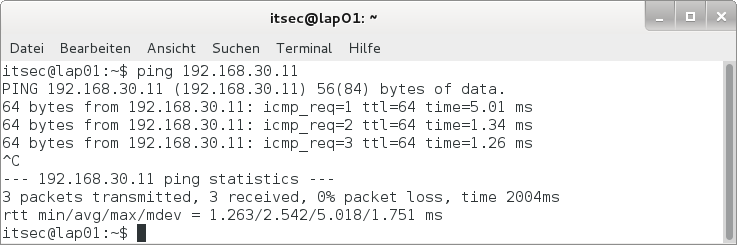
\includegraphics[width=0.7\textwidth]{figures/vpn_lap01_ping_pc01.png}
  \caption{Ping von lap01.internet.f223 mit aktiver VPN zu pc01.firma-a.f223}
  \label{vpn:lap01-ping-pc01}
\end{figure}

\begin{figure}[h!]
  \centering
    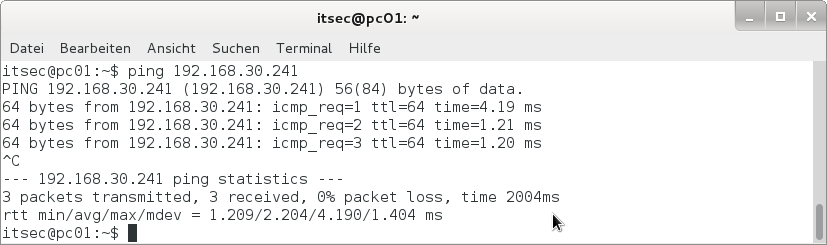
\includegraphics[width=0.7\textwidth]{figures/vpn_pc01_ping_lap01.png}
  \caption{Ping von pc01.firma-a.f223 zu lap01.internet.f223 mit aktiver VPN}
  \label{vpn:pc01-ping-lap01}
\end{figure}

\paragraph{Verschlüsselung der VPN-Verbindung}

\begin{figure}[h!]
  \centering
    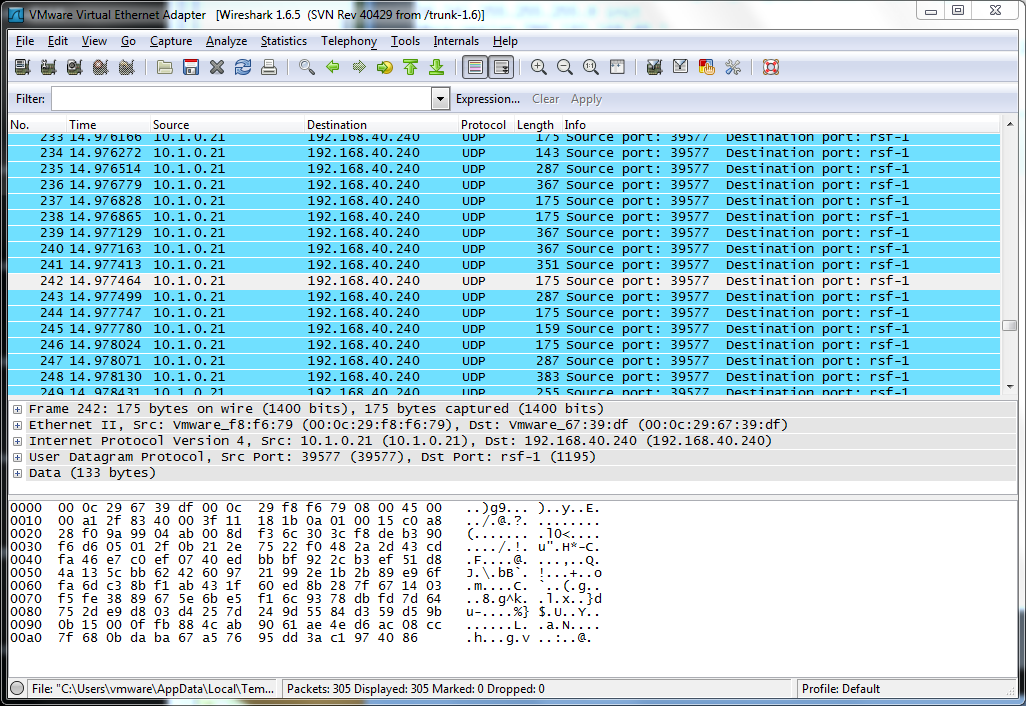
\includegraphics[width=0.7\textwidth]{figures/vpn_ws_lap01_ping_pc01.png}
  \caption{Mitschnitt des Pings von lap01.internet.f223 mit aktiver VPN zu pc01.firma-a.f223}
  \label{vpn:ws_lap01-ping-pc01}
\end{figure}


Um zeigen zu können, dass die Verschlüsselung der VPN-Verbindung funktioniert, wurde ein Mitschnitt der Ping-Nachricht, von lap01 mit aktiver VPN-Verbindung zu pc01, mit Hilfe des Programms Wireshark aufgezeichnet.
Abbildung \ref{vpn:ws_lap01-ping-pc01} zeigt dabei ein Packet des Pings. Hierbei lässt sich gut die Konfiguration erkennen. Als Übertragungsprotokoll wurde UDP verwendet, was die Abbildung bestätigt. Des Weiteren lässt sich zeigen, dass die Packete von lap01 mit dessen öffentlicher IP-Adresse \texttt{10.1.0.21} von einem beliebigen Port \texttt{39577} an den VPN-Server mit der Adresse (DMZ) \texttt{192.168.40.240} an Port \texttt{1195}, welches der konfigurierte Port ist, gesendet werden. Das eigentliche ICMP-Packet an pc01, kann hierbei nicht erkannt werden, da es sich verschlüsselt in diesem Packet befindet.

\paragraph{DNS-Server-Konfiguration}

\begin{figure}[h!]
  \centering
    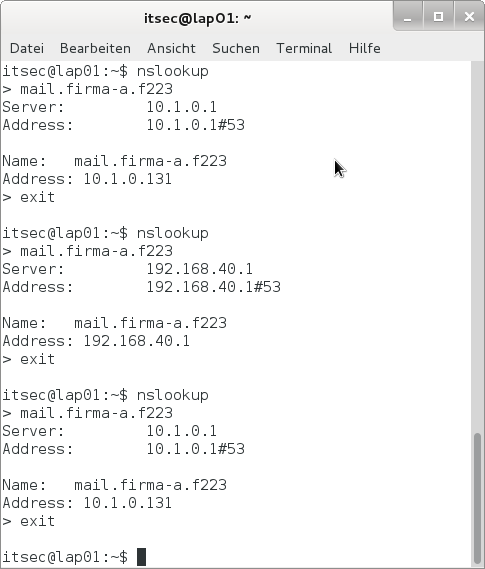
\includegraphics[width=0.5\textwidth]{figures/vpn_nslookup.png}
  \caption{Verifikation der DNS-Server-Konfiguration beim aktivieren der VPN-Verbindung.}
  \label{vpn:lap01_nslookup}
\end{figure}

Abschließend wurde noch die DNS-Server-Konfiguration geprüft, denn wie bereits in Kapitel \ref{vpn:client} erwähnt, soll bei aktiver VPN-Verbindung der Firmeneigene DNS-Server, der sich auf srv01.firma-a.f223 in der DMZ befindet, verwendet werden. Bei nicht aktiver VPN-Verbindung soll der im System konfigurierte DNS-Server auf net1.internet.f223 genutzt werden.

Dies kann mit Hilfe des Programms \texttt{nslookup} verifiziert werden. Der erste, sowie der letzte Aufruf in Abbildung \ref{vpn:lap01_nslookup} erfolgte jeweils mit nicht aktiver VPN-Verbindung. Zum Test wurde die Domain \texttt{mail.firma-a.f223} verwendet, welche in beiden genannten DNS-Servern eingetragen ist.

Hierbei lässt sich erkennen, dass bei nicht aktiver VPN jeweils der DNS-Server mit der IP-Adresse 10.1.0.1 verwendet wurde, sprich der net1 Server. Des Weiteren lässt sich erkennen, dass dieser die Domain auf die äußere IP-Adresse von fw1 auflöst, was korrekt ist.

Der mittlere Eintrag wurde mit aktiver VPN-Verbindung durchgeführt. Hierbei lässt sich erkennen, dass diesmal der Firmeneigenen DNS-Server mit der IP-Adresse \texttt{192.168.40.1} verwendet wird. Zudem löst der DNS-Server die Domain ebenfalls auf diese IP-Adresse auf, da sich der Webserver auf dem gleichen Server befindet.

Durch diese drei Aufrufe wird bestätigt, dass das Ändern und wieder Rückgängig machen, der Änderung des DNS-Servers, beim Aktivieren und Deaktivieren der VPN-Verbindung, funktioniert.
